Redesign the circuit of Fig. \ref{fig:ee18btech11049_fig1} for operation at 10KHz using same values of resistance. If at 10KHz the op amp provides an excess phase shift (lag) of 5.7\degree , what will be the frequency of oscillation? Assume the phase shift introduced by the op amp remains constant for frequencies around 10KHz.)To restore operation to 10KHz, what change must be made in the shunt resistor of the wien bridge? Also, to what value must $R_{2}/R_{1}$ be changed ?
\begin{figure}[!ht]
	\begin{center}
		\resizebox{\columnwidth}{!}{\begin{circuitikz}[scale = 1]
\draw
(0,0) to[empty diode] (4,0) -- (4,1.5)
    to[R, *-*,l_ = $10k\Omega$] (0,1.5) -- (0,0)
(4,1.5) -- (4,3)
    to[empty diode] (0,3) -- (0,1.5)
    to[vR, l_ = $50k\Omega$] (-4,1.5) 
    to (-4,1) node[ground]{} 
(-0.8,1.5) -- (-0.8,4) -- (4,4)
    node[ocirc]{Vo}
(-2,1.2) -- (-2,-2)
 (2.8,-2.5) node[op amp] (opamp) {}
 (opamp.-) -- (-2,-2)
 (opamp.+) -- (-1,-3) -- (-1,-4.5)
 to[C, l= C,*-*] (2,-4.5)to[R,l_=R] (4,-4.5) 
 to (opamp.out) to (4,0)

(-1,-4.5) to[R,l = R] (-1,-7) to  (-1,-7) node[ground]{} 
(-1,-4.5) to[C,l = C] (-3,-4.5) to  (-3,-4.5) node[ground]{} 


;
\end{circuitikz}




}
	\end{center}
\caption{}
\label{fig:ee18btech11049_fig1}
\end{figure}
\begin{enumerate}[label=\arabic*.,ref=\theenumi]
%\begin{enumerate}[label=\thesection.\arabic*.,ref=\thesection.\theenumi]
\numberwithin{equation}{enumi}

\item Draw block diagram for the above circuit .
\\
\solution  
\begin{figure}[!ht]
	\begin{center}
		\resizebox{\columnwidth}{!}{\tikzstyle{block} = [draw, fill=blue!20, rectangle, 
    minimum height=3em, minimum width=6em]
\tikzstyle{sum} = [draw, fill=blue!20, circle, node distance=1cm]
\tikzstyle{input} = [coordinate]
\tikzstyle{output} = [coordinate]
\tikzstyle{pinstyle} = [pin edge={to-,thin,black}]

\begin{tikzpicture}[auto, node distance=2cm,>=latex']
    \node [input, name=input] {};
    \node [sum, right of=input] (sum) {};
    \node [block, right of=sum] (controller) {$G$};
    \node [output, right of=controller] (output) {};
    \node [block, below of=controller] (feedback) {$H$};
    \draw [draw,->] (input) -- node {} (sum);
    \draw [->] (sum) -- node {$V_i$} (controller);
    \draw [->] (controller) -- node [name=y] {$V_o$}(output);
    \draw [->] (y) |- (feedback);
    \draw [->] (feedback) -| node[pos=0.99]{$+$}  node [near end] {$V_f$} (sum);
\end{tikzpicture}
}
	\end{center}
\caption{}
\label{fig:ee18btech11049_block}
\end{figure}

\item Find G and draw circuit diagram for G .  
\\
\solution  
\begin{figure}[!ht]
	\begin{center}
		\resizebox{\columnwidth}{!}{\usetikzlibrary{decorations.markings}
\begin{circuitikz}
\ctikzset{bipoles/length=1cm}

\draw 
% (1.5,1)  to [R=$R_{11}$,*-*] (0,1) to (0,-1)  node[ground]{} 
%(1.5,2) to [R=$R$] (3,2) to [R=$R$] (3,4) to (3,5) node[ground,rotate=180]{} 
%(3,2) --  (4.5,2) to [C=$C$](4.5,4) to (4.5,5) node[ground,rotate=180]{}
%(1.5,3) node[pos=10]{$V_i$}
(1.5,-1.25)  node at(1.7,-1.25){$-$} 
(1.5,-1.25) -- (1,-1.25) -- (1,-1.75) to[R=$R_1$] (1,-2.75) --(1,-3) node[ground]{}
(1,-1.5) to[R=$R_2$,*-*] (5,-1.5) {}
(5,-1.5) -- (5,1) --(3.5,1) to[V=$A_{0}V_i$] (3.5,-0.5) node[ground]{}
(5,1) --(6,1)
(6,1) --(6,1) node at(6.3,1){$V_o$}
node at (1.8,-0.3) {$V_i$}  
node at (1.4,1.3) {$V_{f}$}
node at (0.65,-1.5){$V_{f2}$}
node at(1.8,1){$+$}
;\end{circuitikz}
}
	\end{center}
\caption{}
\label{fig:ee18btech11049_g_block}
\end{figure}

from fig. \ref{fig:ee18btech11049_g_block} 

\begin{align}
    V_{f2} = \brak{\frac{R_1}{R_1 + R_2}}V_o
\end{align}
\begin{align}
    G_1 = \frac{V_{f2}}{V_o} = \brak{\frac{R_1}{R_1 + R_2}}
\end{align}
from fig \ref{fig:ee18btech11049_g_block} , $A_o$ is the gain of amplifier, and $G_1$ is placed as negative feedback factor. Therefore total G is given as

\begin{align}
G &= \frac{A_{0}}{1+A_{0}G_{1}}
\\
&= \frac{1}{\frac{1}{A_{0}} + G_{1}}
\\
\implies G&\approx \frac{1}{G_{1}}, \quad   A_{0}\to\infty
\\
\text{or, } G &= \frac{R_{1}+R_{2}}{R_{1}}=1+\frac{R_{2}}{R_{1}}
\label{eq:ee18btech11047_G}
\end{align}


\item  Find H and draw circuit diagram for H
\\
\solution  

\begin{figure}[!ht]
	\begin{center}
		\resizebox{\columnwidth}{!}{\begin{circuitikz}[scale=.8]
\draw
(0,0) to[C,*-*, l = C] (3,0)
    to[R,*-*,l = R] (6,0)
    node[ocirc]{V2}
(0,0) -- (-4,0)
    node[ocirc]{V1}

(0,0) to[R, l = R] (0,-3) node[ground]{} 
(-2,0) to[C, l_ = C] (-2,-3) node[ground]{} 

;
\end{circuitikz}
}
	\end{center}
\caption{}
\label{fig:ee18btech11049_h_block}
\end{figure}

from fig \ref{fig:ee18btech11049_h_block} 
\begin{align}
    V_1 = \frac{R \parallel \frac{1}{sC}}{\brak{R \parallel \frac{1}{sC}} + R + \frac{1}{sC}} V_2
\end{align}
\begin{align}
    H = \frac{1}{3+j\brak{\omega CR - 1/\omega CR}}
\end{align}



\item Find frequency of oscillation when the excess phase shift \brak{lag} is 5.7\degree
\\
\solution  The loop gain of wein bridge oscillator$L\brak{j\omega}$ is 


\begin{align}
    L\brak{j\omega} = H\brak{j\omega}G\brak{j\omega}
\end{align}
%
\begin{align}
\label{eq:ee18btech11049_wein_main}
    L\brak{j\omega} = \frac{1+ R_2/R_1 }  {3+j\brak{\omega CR - 1/\omega CR}}
\end{align}
%
The phase shift of loop is 
\begin{align}
\label{eq:ee18btech11049_loop_phase}
    \phi\brak{\omega} = \tan^{-1}\brak{\frac{\omega CR - 1/\omega CR}{3}}
\end{align}
%
The loop gain will be a real number
(i.e., the phase will be zero) at the frequency

\begin{align}
\label{eq:ee18btech11049_freq}
    \omega = \frac{1}{CR}
\end{align}
%
Differentiating $\phi\brak{\omega} $ with $\omega$

%
\begin{align}
\label{eq:ee18btech11049_freq}
    \frac{\partial \phi\brak{\omega}}{\partial \omega}
    =\frac{-1}{1+\brak{\frac{\omega CR - 1/\omega CR}{3}}^2}
    \frac{\partial \brak{\omega CR - 1/\omega CR }}{\partial \omega}
\end{align}

%
And since $\omega = 1/CR$ upon evaluating  

%
\begin{align}
\label{eq:ee18btech11049_freq}
    \frac{\partial \phi\brak{\omega}}{\partial \omega}
   = \frac{-2CR}{3} = \frac{-2}{3\omega}
\end{align}
%
\begin{align}
\label{eq:ee18btech11049_freq}
    \text{and } \Delta\omega = \frac{\Delta\phi}{ \frac{\partial \phi\brak{\omega}}{\partial \omega}}
\end{align}

\begin{align}
\label{eq:ee18btech11049_freq}
    \Delta\omega = \frac{-0.1}{ -2/3\omega} \brak{ 5.7\degree = 0.1 rad/s }
\end{align}

\begin{align}
\label{eq:ee18btech11049_freq}
    \Delta\omega = 0.15\omega
\end{align}
%
So, the frequency of oscillation is 
\begin{align}
\label{eq:ee18btech11049_freq}
    \omega - \Delta\omega = 10-0.15x10\\ 
    = 8.15 kHz
\end{align}

\item What change must be made in the shunt resistor of the wien bridge, to restore the frequency of oscillation ? \\
\solution Assuming the parallel R = $R_s$ as shunt shown in Fig \ref{fig:ee18btech11049_fig2}

\begin{figure}[!ht]
	\begin{center}
		\resizebox{\columnwidth}{!}{\begin{enumerate}[label=\thesection.\arabic*.,ref=\thesection.\theenumi]
\numberwithin{equation}{enumi}

\item
For the unity feedback system shown in Fig. \ref{fig:ee18btech11049_block_1} , with 
\begin{align}
    G(s) = \frac{K}{s(s+1)(s+4)}
\end{align}
Design a lag-lead
compensator to yield a  $K_{v} = 12$ as well as peak overshoot
of 12\% and peak time of less than or equal to 2 seconds.
\begin{figure}[!ht]
\begin{center}
	\resizebox{\columnwidth}{!}{.%\begin{figure}
\tikzstyle{block} = [draw, fill=blue!20, rectangle, 
    minimum height=1cm, minimum width=2cm]
\tikzstyle{sum} = [draw, fill=blue!20, circle, node distance=1cm]
\tikzstyle{input} = [coordinate]
\tikzstyle{output} = [coordinate]
\tikzstyle{pinstyle} = [pin edge={to-,thin,black}]

% The block diagram code is probably more verbose than necessary
\begin{tikzpicture}[auto, node distance=3cm,>=latex']
    % We start by placing the blocks
    \node [input, name=input] {X(s)};
    \node [sum, right of=input] (sum) {};
    \node [block, right of=sum] (controller) {G(s)};
    \node [block, right of=controller] (system) {$G_c(s)$};
    % We draw an edge between the controller and system block to 
    % calculate the coordinate u. We need it to place the measurement block. 
    \draw [->] (controller) -- node[name=u] {} (system);
    \node [output, right of=system] (output) {};
    \node [block, below of=u] (measurements) {1};

    % Once the nodes are placed, connecting them is easy. 
    \draw [draw,->] (input) -- node {$X(s)$} (sum);
    \draw [->] (sum) -- node {} (controller);
    \draw [->] (system) -- node [name=y] {$Y(s)$}(output);
    \draw [->] (y) |- (measurements);
    \draw [->] (measurements) -| node[pos=0.99] {$-$} 
        node [near end] {} (sum);
\end{tikzpicture}
%\end{figure}}
\end{center}
    \caption{}
    \label{fig:ee18btech11049_block_1}
\end{figure}

\item
\solution

\begin{align}
    K_{v} = \lim_{s \to 0} s G(s) = 12\\
    \implies K = 48
\end{align}
The bode plot for G(s)is as follows : 

\begin{align}
    G(s) = \frac{48}{s(s+1)(s+4)}
\end{align}

\begin{figure}[!h]
    \centering
    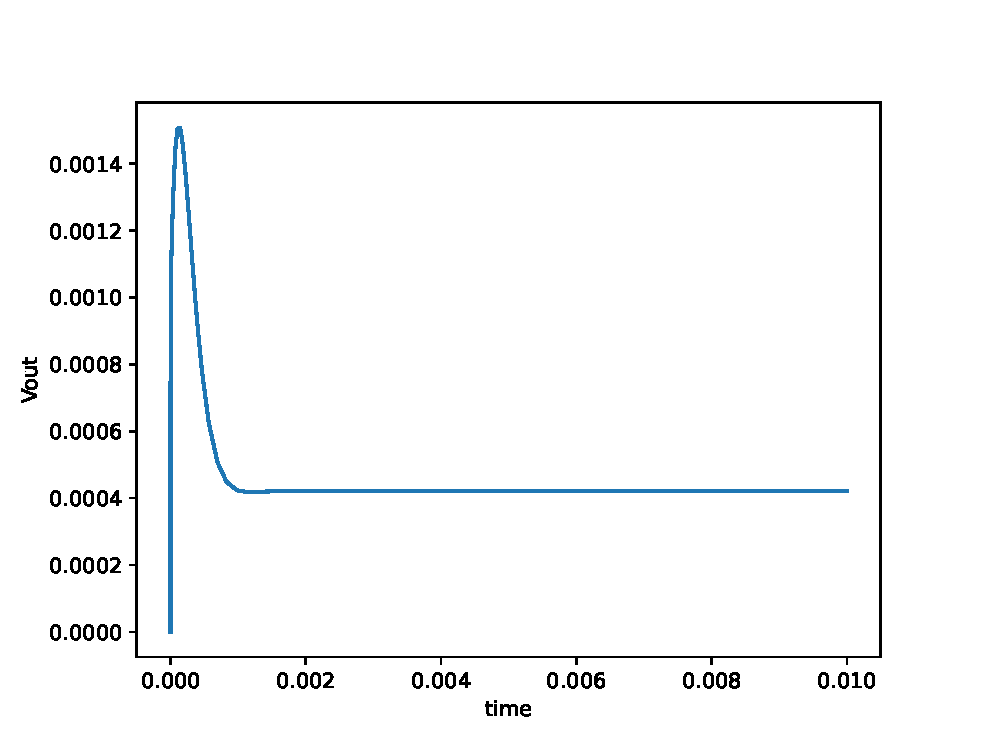
\includegraphics[width=\columnwidth]{./figs/ee18btech11049/ee18btech11049_1.eps}
    \caption{G(s) Bode Plot}
    \label{fig:ee18btech11049_1}
\end{figure}

Damping Ratio $\zeta$
\begin{align}
    \zeta = \frac{-\ln\left(\frac{OS\%}{100}\right)}{\sqrt{\pi^2+\left(\ln\left(\frac{OS\%}{100}\right)\right)^2}}
\end{align}
Phase Margin $\phi_{M}$
\begin{align}
    \phi_{M} = \tan^{-1}\left(\frac{2\zeta}{\sqrt{-2\zeta^2 + \sqrt{4\zeta^4 + 1}}}\right)  
\end{align}
closed-loop Bandwidth $\omega_{bw}$
\begin{align}
    \omega_{bw} = \frac{\pi}{T_{p}\sqrt{1-\zeta ^2}}\sqrt{1-2\zeta^2+\sqrt{4\zeta^4 - 4\zeta ^2 + 2}}
\end{align}

The following code computes the above quantities.
\begin{lstlisting}
codes/ee18btech11049/ee18btech11049_1.py
\end{lstlisting}
\begin{align}
    \zeta  =  0.557\\
    \phi_{M} = 56.13\degree\\
     \omega_{bw} = 2.27 \text{ rad/sec }
\end{align}{}



The required phase margin to yield a 12\% OS is 56.13\degree \\
Let us select  $\omega = $1.83 rad/s as the new phase-margin frequency. \\At this frequency, the uncompensated phase is -176 and would require, if we
add a -6 contribution from the lag compensator, a +56 contribution from the
lead compensator.

\begin{align}
    G_{Lead}\brak{s}G_{Lag}\brak{s} = \left(\frac{s+\frac{1}{T_1}}{s+\frac{\gamma}{T_1}}\right)\left(\frac{s+\frac{1}{T_2}}{s+\frac{1}{\gamma T_2}}\right)
\end{align}

Choose the lag compensator 1-decade below, so that its
will have minimal effect at the new phase-margin frequency.
\begin{align}
     \phi_{max,lead} = 56 = \sin^{-1}{\frac{1-\beta}{1+\beta}}
\end{align}
\begin{align}
    \beta = 0.092 
\end{align}
\begin{align}
      \gamma = 10.86 \text{   since  } \gamma = \frac{1}{\beta}
\end{align}
Thus with $\gamma$ = 10.86 
\begin{align}
    G_{Lag}\brak{s} = \left(\frac{s+\frac{1}{T_2}}{s+\frac{1}{\gamma T_2}}\right)=  \frac{s+0.183}{s+0.0168}
\end{align}
\begin{align}
    \omega_{max} = \frac{1}{T_1 \sqrt{\beta}}
\end{align}

Using Values of $\omega_{max}  = 1.83 $ and $\beta = 0.094$
\begin{align}
     G_{Lag}\brak{s} = \left(\frac{s+\frac{1}{T_1}}{s+\frac{\gamma}{T_1}}\right) = \frac{s+0.55}{s+5.69}
\end{align}

The lag-lead Compensated System's open loop transfer function is
\begin{align}
  G_{total}\brak{s} =  \frac{48\brak{s+0.183}\brak{s+0.55}}{s\brak{s+1}\brak{s+4}\brak{s+0.0168}\brak{s+5.69}}
\end{align}
\begin{figure}[!h]
    \centering
    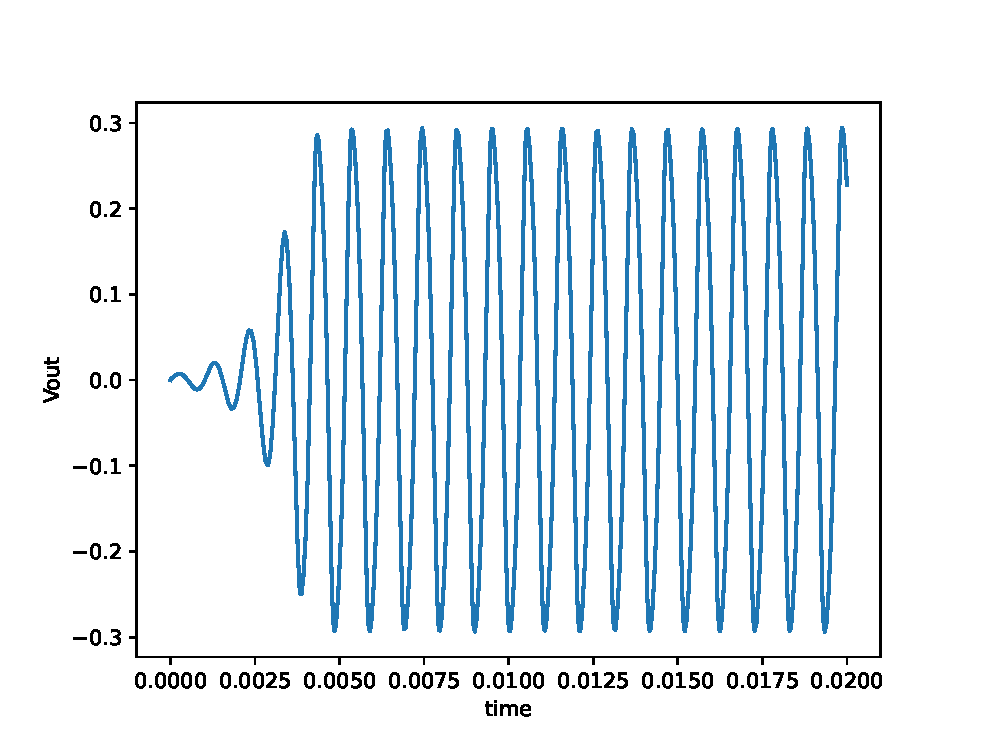
\includegraphics[width=\columnwidth]{./figs/ee18btech11049/ee18btech11049_2.eps}
    \caption{G(s) Compensated Bode Plot}
    \label{fig:ee18btech11049_2}
\end{figure}


\item
\textbf{Verification : }
We could observe the  affect of the lag-lead  compensator from these phase plots.\\

\begin{figure}[!h]
    \centering
    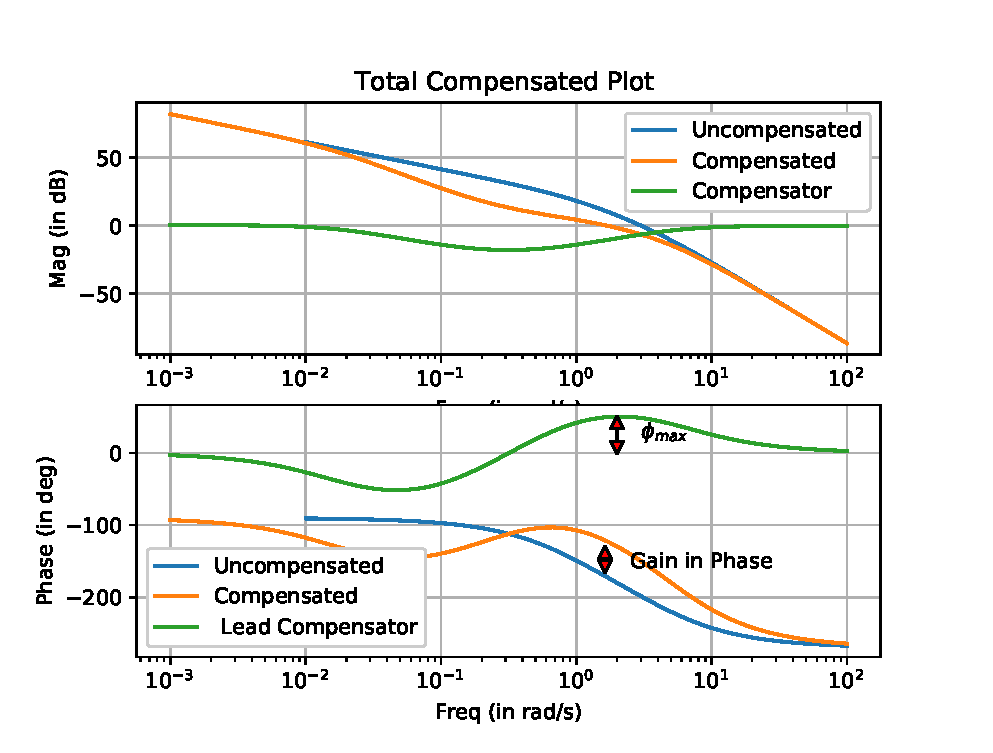
\includegraphics[width=\columnwidth]{./figs/ee18btech11049/ee18btech11049_3.eps}
    \caption{Combined Bode Plots}
    \label{fig:ee18btech11049_3}
\end{figure}






These plots are generated using the below code:
\begin{lstlisting}
codes/ee18btech11049/ee18btech11049_2.py
\end{lstlisting}
\item
\textbf{Result :}
The below is the summary for the designed lead-lead compensator.\\

\begin{table}[!ht]
\centering
%%%%%%%%%%%%%%%%%%%%%%%%%%%%%%%%%%%%%%%%%%%%%%%%%%%%%%%%%%%%%%%%%%%%%%
%%                                                                  %%
%%  This is the header of a LaTeX2e file exported from Gnumeric.    %%
%%                                                                  %%
%%  This file can be compiled as it stands or included in another   %%
%%  LaTeX document. The table is based on the longtable package so  %%
%%  the longtable options (headers, footers...) can be set in the   %%
%%  preamble section below (see PRAMBLE).                           %%
%%                                                                  %%
%%  To include the file in another, the following two lines must be %%
%%  in the including file:                                          %%
%%        \def\inputGnumericTable{}                                 %%
%%  at the beginning of the file and:                               %%
%%        \input{name-of-this-file.tex}                             %%
%%  where the table is to be placed. Note also that the including   %%
%%  file must use the following packages for the table to be        %%
%%  rendered correctly:                                             %%
%%    \usepackage[latin1]{inputenc}                                 %%
%%    \usepackage{color}                                            %%
%%    \usepackage{array}                                            %%
%%    \usepackage{longtable}                                        %%
%%    \usepackage{calc}                                             %%
%%    \usepackage{multirow}                                         %%
%%    \usepackage{hhline}                                           %%
%%    \usepackage{ifthen}                                           %%
%%  optionally (for landscape tables embedded in another document): %%
%%    \usepackage{lscape}                                           %%
%%                                                                  %%
%%%%%%%%%%%%%%%%%%%%%%%%%%%%%%%%%%%%%%%%%%%%%%%%%%%%%%%%%%%%%%%%%%%%%%



%%  This section checks if we are begin input into another file or  %%
%%  the file will be compiled alone. First use a macro taken from   %%
%%  the TeXbook ex 7.7 (suggestion of Han-Wen Nienhuys).            %%
\def\ifundefined#1{\expandafter\ifx\csname#1\endcsname\relax}


%%  Check for the \def token for inputed files. If it is not        %%
%%  defined, the file will be processed as a standalone and the     %%
%%  preamble will be used.                                          %%
\ifundefined{inputGnumericTable}

%%  We must be able to close or not the document at the end.        %%
    \def\gnumericTableEnd{\end{document}}


%%%%%%%%%%%%%%%%%%%%%%%%%%%%%%%%%%%%%%%%%%%%%%%%%%%%%%%%%%%%%%%%%%%%%%
%%                                                                  %%
%%  This is the PREAMBLE. Change these values to get the right      %%
%%  paper size and other niceties.                                  %%
%%                                                                  %%
%%%%%%%%%%%%%%%%%%%%%%%%%%%%%%%%%%%%%%%%%%%%%%%%%%%%%%%%%%%%%%%%%%%%%%

    \documentclass[12pt%
              %,landscape%
                    ]{report}
       \usepackage[latin1]{inputenc}
       \usepackage{fullpage}
       \usepackage{color}
       \usepackage{array}
       \usepackage{longtable}
       \usepackage{calc}
       \usepackage{multirow}
       \usepackage{hhline}
       \usepackage{ifthen}

    \begin{document}


%%  End of the preamble for the standalone. The next section is for %%
%%  documents which are included into other LaTeX2e files.          %%
\else

%%  We are not a stand alone document. For a regular table, we will %%
%%  have no preamble and only define the closing to mean nothing.   %%
    \def\gnumericTableEnd{}

%%  If we want landscape mode in an embedded document, comment out  %%
%%  the line above and uncomment the two below. The table will      %%
%%  begin on a new page and run in landscape mode.                  %%
%       \def\gnumericTableEnd{\end{landscape}}
%       \begin{landscape}


%%  End of the else clause for this file being \input.              %%
\fi

%%%%%%%%%%%%%%%%%%%%%%%%%%%%%%%%%%%%%%%%%%%%%%%%%%%%%%%%%%%%%%%%%%%%%%
%%                                                                  %%
%%  The rest is the gnumeric table, except for the closing          %%
%%  statement. Changes below will alter the table's appearance.     %%
%%                                                                  %%
%%%%%%%%%%%%%%%%%%%%%%%%%%%%%%%%%%%%%%%%%%%%%%%%%%%%%%%%%%%%%%%%%%%%%%

\providecommand{\gnumericmathit}[1]{#1} 
%%  Uncomment the next line if you would like your numbers to be in %%
%%  italics if they are italizised in the gnumeric table.           %%
%\renewcommand{\gnumericmathit}[1]{\mathit{#1}}
\providecommand{\gnumericPB}[1]%
{\let\gnumericTemp=\\#1\let\\=\gnumericTemp\hspace{0pt}}
 \ifundefined{gnumericTableWidthDefined}
        \newlength{\gnumericTableWidth}
        \newlength{\gnumericTableWidthComplete}
        \newlength{\gnumericMultiRowLength}
        \global\def\gnumericTableWidthDefined{}
 \fi
%% The following setting protects this code from babel shorthands.  %%
 \ifthenelse{\isundefined{\languageshorthands}}{}{\languageshorthands{english}}
%%  The default table format retains the relative column widths of  %%
%%  gnumeric. They can easily be changed to c, r or l. In that case %%
%%  you may want to comment out the next line and uncomment the one %%
%%  thereafter                                                      %%
\providecommand\gnumbox{\makebox[0pt]}
%%\providecommand\gnumbox[1][]{\makebox}

%% to adjust positions in multirow situations                       %%
\setlength{\bigstrutjot}{\jot}
\setlength{\extrarowheight}{\doublerulesep}

%%  The \setlongtables command keeps column widths the same across  %%
%%  pages. Simply comment out next line for varying column widths.  %%
\setlongtables

\setlength\gnumericTableWidth{%
    80pt+%
    50pt+%
    60pt+%
0pt}
\def\gumericNumCols{3}
\setlength\gnumericTableWidthComplete{\gnumericTableWidth+%
         \tabcolsep*\gumericNumCols*2+\arrayrulewidth*\gumericNumCols}
\ifthenelse{\lengthtest{\gnumericTableWidthComplete > \linewidth}}%
         {\def\gnumericScale{\ratio{\linewidth-%
                        \tabcolsep*\gumericNumCols*2-%
                        \arrayrulewidth*\gumericNumCols}%
{\gnumericTableWidth}}}%
{\def\gnumericScale{1}}

%%%%%%%%%%%%%%%%%%%%%%%%%%%%%%%%%%%%%%%%%%%%%%%%%%%%%%%%%%%%%%%%%%%%%%
%%                                                                  %%
%% The following are the widths of the various columns. We are      %%
%% defining them here because then they are easier to change.       %%
%% Depending on the cell formats we may use them more than once.    %%
%%                                                                  %%
%%%%%%%%%%%%%%%%%%%%%%%%%%%%%%%%%%%%%%%%%%%%%%%%%%%%%%%%%%%%%%%%%%%%%%

\ifthenelse{\isundefined{\gnumericColA}}{\newlength{\gnumericColA}}{}\settowidth{\gnumericColA}{\begin{tabular}{@{}p{80pt*\gnumericScale}@{}}x\end{tabular}}

\ifthenelse{\isundefined{\gnumericColB}}{\newlength{\gnumericColB}}{}\settowidth{\gnumericColB}{\begin{tabular}{@{}p{50pt*\gnumericScale}@{}}x\end{tabular}}

\ifthenelse{\isundefined{\gnumericColC}}{\newlength{\gnumericColC}}{}\settowidth{\gnumericColC}{\begin{tabular}{@{}p{60pt*\gnumericScale}@{}}x\end{tabular}}
\begin{tabular}[c]{%
    b{\gnumericColA}%   
    b{\gnumericColB}%
    b{\gnumericColC}%
    }

%%%%%%%%%%%%%%%%%%%%%%%%%%%%%%%%%%%%%%%%%%%%%%%%%%%%%%%%%%%%%%%%%%%%%%
%%  The longtable options. (Caption, headers... see Goosens, p.124) %%
%   \caption{The Table Caption.}             \\ %
% \hline    % Across the top of the table.
%%  The rest of these options are table rows which are placed on    %%
%%  the first, last or every page. Use \multicolumn if you want.    %%

%%  Header for the first page.                                      %%
%   \multicolumn{3}{c}{The First Header} \\ \hline 
%   \multicolumn{1}{c}{colTag}  %Column 1
%   &\multicolumn{1}{c}{colTag} %Column 2
%   &\multicolumn{1}{c}{colTag} \\ \hline %Last column
%   \endfirsthead

%%  The running header definition.                                  %%
%   \hline
%   \multicolumn{3}{l}{\ldots\small\slshape continued} \\ \hline
%   \multicolumn{1}{c}{colTag}  %Column 1
%   &\multicolumn{1}{c}{colTag} %Column 2
%   &\multicolumn{1}{c}{colTag} \\ \hline %Last column
%   \endhead

%%  The running footer definition.                                  %%
%   \hline
%   \multicolumn{3}{r}{\small\slshape continued\ldots} \\
%   \endfoot

%%  The ending footer definition.                                   %%
%   \multicolumn{3}{c}{That's all folks} \\ \hline 
%   \endlastfoot
%%%%%%%%%%%%%%%%%%%%%%%%%%%%%%%%%%%%%%%%%%%%%%%%%%%%%%%%%%%%%%%%%%%%%%


    
\hhline{---}
     \multicolumn{1}{|p{\gnumericColA}|}%
    {\gnumericPB{\centering}\textbf{Specifications}}
    &\multicolumn{1}{p{\gnumericColB}|}%
    {\gnumericPB{\centering}\textbf{Expected}}
    &\multicolumn{1}{p{\gnumericColC}|}%
    {\gnumericPB{\centering}\textbf{Proposed}}

\\

    

\hhline{|---|}
     \multicolumn{1}{|p{\gnumericColA}|}%
    {\gnumericPB{\centering}OS\%}
    &\multicolumn{1}{p{\gnumericColB}|}%
    {\gnumericPB{\centering}12\%}
    &\multicolumn{1}{p{\gnumericColC}|}%
    {\gnumericPB{\centering}10.2\%}
    
    



\\


\hhline{|---|}
     \multicolumn{1}{|p{\gnumericColA}|}%
    {\gnumericPB{\centering}$T_{p}$}
    &\multicolumn{1}{p{\gnumericColB}|}%
    {\gnumericPB{\centering}$<=2$}
    &\multicolumn{1}{p{\gnumericColC}|}%
    {\gnumericPB{\centering} 1.61}


\\

\hhline{|---|}
     \multicolumn{1}{|p{\gnumericColA}|}%
    {\gnumericPB{\centering}$\phi_{M}$}
    &\multicolumn{1}{p{\gnumericColB}|}%
    {\gnumericPB{\centering}56 }
    &\multicolumn{1}{p{\gnumericColC}|}%
    {\gnumericPB{\centering} 59.6}


\\


\hhline{|---|}
     \multicolumn{1}{|p{\gnumericColA}|}%
    {\gnumericPB{\centering}$\omega_{bw}$}
    &\multicolumn{1}{p{\gnumericColB}|}%
    {\gnumericPB{\centering}$>=2.27$}
    &\multicolumn{1}{p{\gnumericColC}|}%
    {\gnumericPB{\centering} 3}

\\
\hhline{|---|}
     \multicolumn{1}{|p{\gnumericColA}|}%
    {\gnumericPB{\centering}$\omega_{gc}$}
    &\multicolumn{1}{p{\gnumericColB}|}%
    {\gnumericPB{\centering}-}
    &\multicolumn{1}{p{\gnumericColC}|}%
    {\gnumericPB{\centering}1.63 }

\\
    
    
    \hhline{|---|}
     \multicolumn{1}{|p{\gnumericColA}|}%
    {\gnumericPB{\centering}$K_{v}$}
    &\multicolumn{1}{p{\gnumericColB}|}%
    {\gnumericPB{\centering}12}
    &\multicolumn{1}{p{\gnumericColC}|}%
    {\gnumericPB{\centering}12}

\\
\hhline{|-|-|-}
\end{tabular}

\ifthenelse{\isundefined{\languageshorthands}}{}{\languageshorthands{\languagename}}
\gnumericTableEnd
\caption{Comparing the desired and obtained results}
\label{table:ee18btech11049_table_1}
\end{table}








\end{enumerate}
}
	\end{center}
\caption{}
\label{fig:ee18btech11049_fig2}
\end{figure}

Feedback loop gain $\beta\brak{s}$

\begin{align}
\label{eq:ee18btech11049_beta}
    \beta\brak{s} = \frac{R_s \parallel \frac{1}{sC}}{\brak{R_s \parallel \frac{1}{sC}} + R + \frac{1}{sC}}
\end{align}

\begin{align}
\label{eq:ee18btech11049_freq}
    \beta\brak{s} = \frac{1}{2 + \frac{R}{R_s} + j\brak{\omega CR - \frac{1}{\omega CR_s}}}
\end{align}

So, phase shift $\phi\brak{\omega}$ is

\begin{align}
\label{eq:ee18btech11049_phase_mine}
    \phi\brak{\omega}  = -\tan^{-1}\brak{\frac{\omega CR - \frac{1}{\omega CR_s}}{2+\frac{R}{R_s}}}
\end{align}

from \ref{eq:ee18btech11049_phase_mine} we can find value of $R_s$ when $\omega = \frac{1}{RC}$ 
\begin{align}
   R_s = 0.75R \\
   R_s = 7.5k\Omega 
\end{align}


\item Also, to what value must $R_2/R_1$ be changed ?
\\
\\
\solution Substituting the values of $R $ and $ R_s$ in \ref{eq:ee18btech11049_beta} we get
\begin{align}
    \beta\brak{j\omega} = \frac{1}{3.35}
\end{align}
%

we know the loop gain $L\brak{j\omega}$ is


\begin{align}
    L\brak{j\omega} = \frac{1+R_2/R_1}{\beta \brak{j\omega}}
\end{align}
Condition for oscillation is $1-L\brak{s} = 0$

\begin{align}
    1 + \frac{R_2}{R_1} = 3.35 \\
    \frac{R_2}{R_1} = 2.35
\end{align}
\end{enumerate}
